%% ----------------------------------------------------------------
%% Thesis.tex -- MAIN FILE (the one that you compile with LaTeX)
%% ---------------------------------------------------------------- 

% Set up the document
\documentclass[a4paper, 11pt, oneside]{Thesis}  % Use the "Thesis" style, based on the ECS Thesis style by Steve Gunn
\graphicspath{Figures/}  % Location of the graphics files (set up for graphics to be in PDF format)

% Include any extra LaTeX packages required
\usepackage[square, numbers, comma, sort&compress]{natbib}  % Use the "Natbib" style for the references in the Bibliography
\usepackage{verbatim}  % Needed for the "comment" environment to make LaTeX comments
\usepackage{vector}  % Allows "\bvec{}" and "\buvec{}" for "blackboard" style bold vectors in maths
\hypersetup{urlcolor=blue, colorlinks=true}  % Colours hyperlinks in blue, but this can be distracting if there are many links.

%% ----------------------------------------------------------------
\begin{document}
\frontmatter      % Begin Roman style (i, ii, iii, iv...) page numbering

% Set up the Title Page
\title  {Reverse Engineering Object-Oriented Systems into Umple: An Incremental and Rule-Based Approach}
\authors  {\texorpdfstring
            {\href{mgarzon@uottawa.ca}{Miguel A. Garz\'{o}n Torres}}
            {Miguel A. Garz\'{o}n}
            }
\date       {\today}
\subject    {}
\keywords   {}

\maketitle
%% ----------------------------------------------------------------

\setstretch{1.3}  % It is better to have smaller font and larger line spacing than the other way round

% Define the page headers using the FancyHdr package and set up for one-sided printing
\fancyhead{}  % Clears all page headers and footers


\rhead{\thepage}  % Sets the right side header to show the page number
\lhead{}  % Clears the left side page header

\pagestyle{fancy}  % Finally, use the "fancy" page style to implement the FancyHdr headers

%% ----------------------------------------------------------------
% The "Funny Quote Page"
\pagestyle{empty}  % No headers or footers for the following pages

\null\vfill
% Now comes the "Funny Quote", written in italics
\textit{''Simplicity is a great virtue but it requires hard work to achieve it and education to appreciate it. And to make matters worse: complexity sells better.''}

\begin{flushright}
Edsger W. Dijkstra
\end{flushright}

\vfill\vfill\vfill\vfill\vfill\vfill\null
\clearpage  % Funny Quote page ended, start a new page
%% ----------------------------------------------------------------

% The Abstract Page
\addtotoc{Abstract}  % Add the "Abstract" page entry to the Contents
\abstract{
\addtocontents{toc}{\vspace{1em}}  % Add a gap in the Contents, for aesthetics

This thesis investigates a novel approach to reverse engineering, in which modeling information such as UML associations, state machines and attributes is incrementally added to code written in Java or C++, while maintaining the system in a textual format. Umple is a textual representation that blends modeling in UML with programming language code. The approach, called umplification, produces a program with behavior identical to the original one, but written in Umple and enhanced with model-level abstractions. As the resulting program is Umple code, our approach eliminates the distinction between code and model. In this paper we discuss the principles of Umple, the umplification approach and a rule-driven tool called the Umplificator, which implements and validates the depicted approach. 
The present thesis consists of three main parts. The first part (Chapter 1 and 2) present the research questions and research methodology and introduces Umple and the Umplification concept. The core of our research is presented in Chapters 4 and 5. The last part, Chapter 6, presents details of a case study conducted on an open source software application, JHotDraw. Finally, the expected contributions are listed in Chapter 7.

}

\clearpage  % Abstract ended, start a new page
%% ----------------------------------------------------------------

\setstretch{1.3}  % Reset the line-spacing to 1.3 for body text (if it has changed)

% The Acknowledgements page, for thanking everyone
\acknowledgements{
\addtocontents{toc}{\vspace{1em}}  % Add a gap in the Contents, for aesthetics

A very special, and well-deserved, thank you to the following:

}
\clearpage  % End of the Acknowledgements
%% ----------------------------------------------------------------

\pagestyle{fancy}  %The page style headers have been "empty" all this time, now use the "fancy" headers as defined before to bring them back


%% ----------------------------------------------------------------
\lhead{\emph{Contents}}  % Set the left side page header to "Contents"
\tableofcontents  % Write out the Table of Contents

%% ----------------------------------------------------------------
\lhead{\emph{List of Figures}}  % Set the left side page header to "List if Figures"
\listoffigures  % Write out the List of Figures

%% ----------------------------------------------------------------
\lhead{\emph{List of Tables}}  % Set the left side page header to "List of Tables"
\listoftables  % Write out the List of Tables

%% ----------------------------------------------------------------
\setstretch{1.5}  % Set the line spacing to 1.5, this makes the following tables easier to read
\clearpage  % Start a new page
\lhead{\emph{Glossary}}  % Set the left side page header to "Abbreviations"



%% ----------------------------------------------------------------
\mainmatter	  % Begin normal, numeric (1,2,3...) page numbering
\pagestyle{fancy}  % Return the page headers back to the "fancy" style

% Include the chapters of the thesis, as separate files
% Just uncomment the lines as you write the chapters
\lhead{\emph{\rightmark}} 

\chapter{Introduction}

Many software systems experience growth and change for an extended period of time. Maintaining consistency between documentation and the corresponding code becomes challenging. This situation has long been recognized by researchers, and significant effort has been made to tackle it. Reverse engineering is one of the fruits of this effort and has been defined as the process of creating a representation of the system at a higher level of abstraction [1].

Reverse engineering, in general, recovers documentation from code of software systems. When such documentation follows a well-defined syntax it is often now referred to as a model.  Such models are often represented using UML (Unified Modeling Language), which visually represents the static and dynamic characteristics of a system. 

There is a long and rich literature in reverse engineering [2]. Most existing techniques result in the generation of documentation that can be consulted separately from the code. Other tech-niques generate models in the form of UML diagrams that are intended to be used for code generation of a new version of the system. The technique discussed in this paper goes one step further: It modifies the source code to add model constructs that are represented textually, but can also be viewed and edited as diagrams. The target language of our reverse engineering process is Umple [3], which adds UML and other constructs textually to Java, C++ and PHP.

We call our approach to reverse engineering a software system umplification. This is a play on words with the concept of ‘amplification’ and also the notion of converting into Umple. In our previous work [4], we have found that umplifying code is reasonably straightforward for someone familiar with Umple, and with knowledge of UML modeling pragmatics. Moreover, we have per-formed manual umplification of several systems, including Umple itself. 

The present thesis focuses on how the umplification process can be performed automatically by a reverse engineering technology. In the next section, we define and explore the concept of umplification. In Section 1.2, we state the research problem addressed by this proposal and list the research questions. In Section 1.3, we present the methodology that we will follow in order to answer our research questions.

\section{Research Questions}

The problem to be addressed in this research is as follows:

Developers currently often work with large volumes of legacy code. Tools exist to allow them to extract models or transform their code in a variety of ways. However doing so tends to result in a system that is quite different in syntax and structure. They are thus inhibited from using reverse engineering tools except to generate documentation. The Umple technology partly solves this problem by allowing incremental addition of modeling constructs into familiar programming language code. This allows developers to maintain the essential ‘familiarity’ with their code as they gradually transform it. Converting to Umple (Umplifica-tion) has been done manually – indeed it was applied to the Umple compiler itself [Lethbridge, et al. 2010a] –  but it ought to have tool support so it can be done in a more automatic, systematic and error-free manner on large systems.
The research questions are as follows:

\begin{enumerate}

\item What transformation technology, transformations and refactoring patterns will work best for umplification?
\item What percentage of code reduction and complexity reduction can we achieve by umplification, and how can we measure the complexity reduction?
\item Overall, what are the benefits of automated or semi-automated umplification as compared to manual umplification or the use of other reverse-engineering or transformation approaches?
\item What should be the architecture, implementation and user interface of an umplification tool?

\end{enumerate}

\section{Hypothesized Solutions}


\section{Research Activities}

The major steps in the methodology are the following:
\begin{enumerate}
\item 	Manually perform umplification to gain an understanding of what will be needed
\item 	Iteratively develop The Umplificator tool, exploring the effectiveness of various reusable components and transformation approaches. This includes selection or creation of an easy-to-use tool to express transformations from the base language to Umple. We want to avoid complex XML-based solutions since usability will be key.
\item 	Start with a major case study (JHotDraw), iteratively umplifying it and improving the Umplificator until the Umple version of the case study compiles and a significant number of constructs have been umplified successfully
\item 	Iteratively develop more and more transformations to convert additional Java code into Umple. Introduce additional case studies until the Umplificator works well on 10-15 reasonably large open-source systems.
\item 	Compare the work to alternative approaches.
\end{enumerate}

\section{Thesis Contributions}
\section{Outline}
This thesis proposal is organized as follows.

\begin{description}
  \item[Chapter 2] \hfill \\
Chapter 2 presents background research, a brief introduction to Umple and its mod-eling constructs. Additionally, it reviews related and relevant work; by understanding the existing technologies and research on the topic we should be able to efficiently navigate our research topics.  Covered in this chapter are existing technologies in reverse engineering and model-to model transformations. 
  \item[Chapter 3] \hfill \\
Chapter 3 presents umplification in detail, the core of this thesis. 
  \item[Chapter 4] \hfill \\
Chapter 4 presents three different technologies that were explored as part of our re-search activities. We evaluate ATL, TXL and JDT to see to which extent they could fulfill our needs. ATL and TXL are two famous model-to-model transformation technologies and JDT is a complete Java Framework used as part of the Eclipse IDE. We discuss all the design decisions and propose a set of tools and technologies that our prototype tool will use. Design and implementation decisions are not final and will be enhanced as our research progresses.
    \item[Chapter 5] \hfill \\
Chapter 5 presents an analysis of our reverse engineering technique, the design approaches and our prototype tool. We also present the mapping rules employed to perform the transformations.    
    \item[Chapter 6] \hfill \\
Chapter 6 presents the case study conducted to evaluate the feasibility and efficiency of our approach. The case study shows the results of the umplification performed to the JHotDraw framework, we measure lines of code to compare the original system and the umplified version of the system. 
    \item[Chapter 7] \hfill \\
Chapter 7 concludes this proposal by listing all the research contributions expected out of our research. We also summarize our research activities and give and outline of our direction for the final thesis.
\end{description}


 % Introduction

\lhead{\emph{\leftmark}}  % Set the left side page header to "Abbreviations"
\chapter{Background}

This chapter presents the required background knowledge for readers to fully understand the following chapters. We introduce the Umple language and we present the most important concepts about model-to-model transformations and some of the most relevant reverse engineering techniques. 
\section{Umple Modeling Language}

Umple [3] is an open-source textual modeling and programming language that adds UML abstractions to base programming languages including Java, PHP, C++ and Ruby.\\
Umple has been designed to be general purpose and has UML class diagrams and UML state diagrams as its central abstractions. It has state-of-the art code generation and can be used incrementally, meaning that it is easy for developers to gradually switch over to modeling from pure programming. Umple was designed for modeling and developing large systems and for teaching modeling [8]. Umple is written in itself – the original java version was manually umplified many years ago. That experience was one of the motivations for the current work.
In addition to classes, interfaces and generalizations available in object oriented lan-guages, Umple allows software developers to specify:\\
\begin{enumerate}
 \item 	\textbf{Associations}: As in UML, these specify the links between objects that will exist at run time. Umple supports enforcement of multiplicity constraints and manages referential in-tegrity – ensuring that bidirectional references are consistently maintained in both direc-tions.
 \item 	\textbf{Attributes}: These abstract the concept of instance variables. They can have properties such as immutability, and can be subject to constraints, tracing, and hooks that take actions be-fore or after they are changed.
 \item \textbf{	State Machines}: These also follow UML semantics, and can be considered to be a special type of attributes, subject to events that cause transitions from one value to another. States can have entry or exit actions, nested and possibly parallel substates, and activities that operate in concurrent threads.
 \item 	\textbf{Traits}: A trait is a partial description of a class that can be reused in several different classes, with optional renaming of elements. They can be used to describe re-usable custom patterns.
 \item 	\textbf{Patterns}: Umple currently supports the singleton and immutable patterns, as well as keys that allow generation of consistent code for hashing and equality testing.
 \item 	Aspect Oriented Code Injection: This allows injection of code that can be run before or after methods, including Umple-defined actions on attributes, associations and the ele-ments of state machines. Such code can be used as preconditions and post-conditions or for various other purposes. Code can be injected into the API methods (those methods generated by Umple) as well as into user-defined methods. 
 \item 	\textbf{Tracing}:  A sublanguage of Umple called MOTL (Model-oriented tracing language) al-lows developers to specify tracing at the model level, for example to enabling understand-ing of the behavior of a complex set of state machines operating in multiple threads and class instances [9].
 \item 	\textbf{Constraints}: Invariants, preconditions and postconditions can be specified.
 \item 	\textbf{Concurrency}: Umple provides several mechanisms to allow concurrency to be specified easily, including active objects, queuing in state machines, ports, and the aforementioned state activities.
The umplification method discussed in this paper currently focuses on associations and attributes, with some generation of Umple’s patterns and code injections. As future work it is planned to extend it to encompass other Umple features.
\end{enumerate}
The Umple compiler supports code generation for Java, PHP, Ruby, C++ as well as ex-port to XMI and other UML formats. The compiler generates various types of methods in-cluding mutator, accessor, and event methods from the various Umple features. A mutator (e.g. set(), add()) method is a method used to control changes to a variable and an accessor (e.g. get()) method is the one used to return values of the variable. An event method triggers state change. An extended summary of the API generated by Umple from attributes, associa-tions, state machines and other features can be found at [10]. Umple can also generate dia-grams, metrics, and various other self-documentation artifacts. Umple models can be created or edited using the UmpleOnline Web tool [11], the command line compiler or an Eclipse plugin. 
In the following chapter, we will describe the core concept of this thesis proposal, the umplification technique, a model-transformation technique that aims at incrementally trans-forming base language code into Umple code. Later, we will discuss which of the above lan-guages proved most useful for umplification.


\section{Reverse Engineering} % Background  

\lhead{\emph{\leftmark}}  % Set the left side page header to "Abbreviations"
\chapter{Reverse Engineering of Object Oriented Systems into Umple}

Developers often work with large volumes of legacy code. Reverse engineering tools allow them to extract models in a variety of ways [5], often with UML as the resulting formalism.
The extracted models can be temporary, just-in-time aids to understanding, to be discarded after being viewed. Such a mode of use can be useful, but is limited in several ways: Devel-opers still need to know where to start exploring the system, and they need to remember how to use the reverse engineering tool every time they per-form an exploration task. \\
Developers generally therefore would benefit from choosing reverse engineering tools that create a more permanent form of documentation that can be annotated or embedded in larger documents, and serve as the definitive description of the system. \\
However by making the latter choice, the developer then needs to maintain two different artifacts, the original code and the output model. The recovered models become obsolete quickly, unless they are continuously updated or are used for ‘roundtrip engineering’.  The complexity of this inhibits developers from using reverse engineering tools for permanent documentation.\\
The umplification technique we present in this paper overcomes the problems with either mode of reverse engineering described above. It results in a system with a model that can be explored as easily as with just-in-time tools. But there is also no issue with maintaining the model, because model and code become the same thing.\\
In other words, the key difference compared to existing reverse engineering techniques is that the end-product of umplification is not a separate model, but a single artifact seen as both the mod-el and the code. In the Umple world, modeling is programming and vice versa. More specifically, for a programmer, Umple looks like a programming language and the Umple code can be viewed as a traditional UML diagram. This allows developers to maintain the essential ‘familiarity’ with their code as they gradually transform it into Umple [6]. 
In addition to solving the problem of having two different software artifacts to maintain,   umplification can be used to simplify a system. The resulting Umple code base tends to be simpler to understand [7] as the abstraction level of the program has been ‘amplified’.


\section{Umplification Process}
Umplification involves recursively modifying the Umple model/code to incorporate addition-al abstractions, while maintaining the semantics of the program, and also maintaining, to the greatest extent possible, such elements as layout. The end product of umplification is an Umple program/model that can be edited and viewed textually just like the original program, and also diagrammatically, using Umple’s tools. 
The umplification process has several properties. It is:
\begin{enumerate}
 \item incremental, 
 \item transformational,
 \item interactive,  
 \item extensible, and
 \item implicit-knowledge conserving. 
\end{enumerate}

The approach is \textbf{incremental} because it can be performed in multiple small steps that produce (quickly) a new version of the system with a small amount of additional modeling information, such as the presence of one new type of UML construct. At each step, the system remains compilable. The approach proceeds incrementally performing additional transformations until the desired level of abstraction is achieved.	These incremental transformations allow for user interaction to provide needed information that may be missing or hard to automatically obtain because the input (the source code) does not follow any of the idioms the automatic umplification tool is yet able to recognize. This characteristic of umplification allows developers, if they wish, to repeatedly re-introspect the transformed program and manually validate each change with an understanding of the incremental purpose of the change.

The approach is \textbf{transformational} because it modifies the original source rather than generating something completely new. It first translates the original language (Java, C++ etc.) to an initial Umple version that looks very much like the original, and then translates step-by-step as more and more modeling constructs are added, replacing original code.

The approach is \textbf{transformational} because the user's feedback may be used to enhance the transformations.

The approach is \textbf{interactive} because it uses the set of transformation rules can be readily extended to refine the transformation mechanism. 

Finally the approach is \textbf{implicit-knowledge} conserving because it preserves code comments, and, where possible, the layout of whatever code is not (yet) umplified. The latter includes as the bodies of algorithmic methods – known as action code in UML.

Taken together, the above properties allow developers to confidently umplify their sys-tems without worrying about losing their mental model of the source code. Developers gain by having systems with a smaller body of source code that are intrinsically self-documented in UML. 

The following gives a summary of the abstract transformations currently implemented.
\begin{description} 
\item[Transformation 0: Initial transformation] 
To start, source files with language L (e.g. Java, C++) code are initially renamed as Umple files, with extension .ump. File, package and data type's inclusions are translated into Umple dependencies by using the depend construct. 
\item [Transformation 1: Transformation of generalization/specialization, dependency, and namespace declarations]
The notation in the base language code for subclassing is transformed into the Umple 'isA' notation. Umple now recognizes the class hierarchy.  Notations representing dependency are transformed into Umple 'depends' clauses, and notations for namespaces or packages are transformed into the Umple 'namespace' directives. At this stage, an Umple program, when compiled should generate essentially identical code to the original program.
\item [Transformation 2: Analysis and conversion of many instance variables, along with the methods that use the variables]
This transformation step is further decomposed into sub-steps depending on the abstract use of the variables. The sub-steps are defined as follows.
   \begin{description}
\item [Transformation 2a: Transformation of variables to UML/Umple attributes]
If variable a is declared in class A and the type of a is one of the primitive types in the base language, then a is transformed into an Umple attribute. Any accessor (e.g. getA()) and mutator (e.g. setA(…)) methods of variable a are transformed as needed to maintain a func-tioning system. In particular, any getter and setter methods in the original system must be adapted to conform to or call the Umple-generated equivalents.
\item [Transformation 2b: Transformation of variables in one or more classes to UML/Umple associations]
If variable a is declared in Class A and the type of a is a reference type B, then a is trans-formed into an Umple Association with ends {a, b}. At the same time, if a variable b in class B is detected that represents the inverse relationship then the association becomes bidirec-tional. The accessor and mutator methods of variable a (and b) are adapted to conform to the Umple-generated methods. Multiplicities and role names are recovered by inspecting both types A and B; this is explained in Section 3.3. 
\item [Transformation 2c: Transformation of variables to UML/Umple state machines]
If a is declared in Class A, has not been classified previously as an attribute or association, has a fixed set of values, and changes in the values are triggered by events, and not by a set method, then a is transformed to a state machine.	We will not cover this aspect of umplification further in this paper, and will leave the focus on attributes and associations.
As mentioned before, as part of each transformation step, the accessor, mutator, iterator and event methods are adapted (refactored) to conform to the Umple generated methods. Table \ref{table:trasnformations} summarizes these additional required refactorings. 
   \end{description}

\end{description}

\begin{table}[htbp]
	\caption{Refactorings to methods required for each transformation}
	\label{table:trasnformations}
    \centering
    \begin{tabularx}{\textwidth}{| X | X |}
    %\begin{tabularx}{\textwidth}{sb}
        \hline
        \rowcolor[HTML]{BBDAFF}
       \textbf{ Transformation case  }   & \textbf{Method Transformations}
        \\ \hline
        \textbf{(0)  Classes }        & None      \\ \hline
        \textbf{(1)  Inheritance}     & None       \\ \hline
        \textbf{2a)  Attributes}      & 
        Accessor (getter) and mutator (setter) methods are removed from the original code 				if they are simple since Umple-generated code replaces them. Custom accessors and 				mutators are refactored so Umple generates code that maintains the original
        semantics.         		\\ \hline
        \textbf{(2b) Associations }   & 
 		Accessor and mutator methods are removed or correctly injected into the umple code.        
		\\ \hline
        \textbf{(2c) State Machines  }  & 
		Methods triggering state change are removed if they are simple (just change state) or 		modified to call Umple-generated event methods. Not covered further in this 					paper       		
\\ \hline
    \end{tabularx}
\end{table}

In the following chapter, we provide a more detailed view of the transformation cases. To help distinguish between Umple and Java code presented in this thesis, the Umple examples appear in dashed borders with grey shading, pure Java examples have solid borders with no shading. Mapping rules (in the Drool language, that we will describe shortly) appear using double line borders with no shading.  % Reverse Engineering

\lhead{\emph{\leftmark}}  

\chapter{Detection Mechanisms for UML/Umple Constructs}


\section{Initial Refactoring}
The first step in umplification (Transformation 0) is to rename the Java/C++ files as .ump files. After this, various syntactic changes are made (Transformation 1) to adapt the code to Umple's notations for various features that are expressed differently in Java and C++. Umple maintains its own syntax for these features so as to be language-independent.
First the base language notation for inheritance (e.g. 'extends' in Java) or interface implementation (e.g. 'implements') is changed into the Umple notation 'isA'. This Umple keyword is used uniformly to represent the generalization relation-ship for classes, interfaces and traits. The same notation is used for all three for flexibility – so that, for example, an interface can be converted to a class with no change to its specializations, or a trait can be generated as a superclass in languages such as C++ where multiple inheritance is allowed.
After this, the dependency notation in the native language (e.g. 'import' in Java) is changed to the 'depend' notation in Umple. Finally 'package' declarations are transformed into Umple namespace declarations. 
Transformations made as part of these first refactoring steps, are one-to-one direct and simple mappings between constructs in the base language and Umple. No methods need changing. The final output after execution of the above transformations, is an Umple model/program that can be compiled in the same manner as the original base language code. At this point, any available test cases may be run to ensure that the pro-gram's semantics are preserved. For instance, the Java code (in file Student.java) shown below:	


\section{Refactoring to Create Attributes}
In this sub-section, we present how member variables possessing certain characteristics are transformed into Umple attributes (Transformation 2a). An Umple attribute is a simple property of an object, but following UML semantics, it is more than just a plain private variable: It is designed to be operated on by mutator methods, and accessed by accessor methods. These methods, in turn can have semantics such as preconditions and tracing injected into them. 
We start by analyzing all instance variables for their presence in constructor and get/set methods and decide whether the member variable is a good candidate to become an Umple attribute [12].  In Table \ref{table:attributes}, we present the developed (programmable) heuristics used for the partial analysis of member variables. The instance variables with a low or very low probability of being attributes are ignored for now. Those with high and medium probability are further analyzed. 

\begin{table}[h]
\caption{Analyzing instance variables for presence in the constructor and getter/setters}
\label{table:attributes}
\centering
\begin{tabular}{@{}cccc@{}}
\toprule
\rowcolor[HTML]{BBDAFF}
\multicolumn{1}{c}{\cellcolor[HTML]{BBDAFF}Constructor} & \multicolumn{1}{c}{\cellcolor[HTML]{BBDAFF}Setter} & \multicolumn{1}{c}{\cellcolor[HTML]{BBDAFF}Getter} & \multicolumn{1}{c}{\cellcolor[HTML]{BBDAFF}\begin{tabular}[c]{@{}c@{}}Attribute\\ (Probability)\end{tabular}} \\ \midrule
Yes                                                     & Yes                                                & Yes                                                & High                                                                                                          \\
Yes                                                     & Yes                                                & No                                                 & Low                                                                                                           \\
Yes                                                     & No                                                 & Yes                                                & High                                                                                                          \\
Yes                                                     & No                                                 & No                                                 & Low                                                                                                           \\
No                                                      & Yes                                                & Yes                                                & High                                                                                                          \\
No                                                      & Yes                                                & No                                                 & Low                                                                                                           \\
No                                                      & No                                                 & Yes                                                & Medium                                                                                                        \\
No                                                      & No                                                 & No                                                 & Very Low                                                                                                      \\ \bottomrule
\end{tabular}
\end{table}

Furthermore, we check the type of the candidate attributes (those with a High or Medium probability) and draw a conclusion regarding whether or not the member variable corresponds to an Umple Attribute, because some will be left to be later transformed into associations. If the candidate attribute has as its type either: a) a simple data type, as in Table \ref{table:attributes2} or b) a class that only itself contains instance variables meeting conditions in a and b (for attributes with 'many' multiplicity), then the member variable is transformed into an Umple Attribute.

\begin{table}
\caption{Umple Primitive Data Types}
\label{table:attributes2}
\centering
    \begin{tabular}{ll}
		\toprule
		\rowcolor[HTML]{BBDAFF}
        \textbf{Type}      & \textbf{Description}                               \\ 
        \hline
        Integer   & Includes signed and unsigned integers.    \\ 
        String    & All string and string builder types       \\ 
        Boolean   & true/false types                          \\ 
        Double    & All decimal object types                  \\ 
        Date/Time & All date, time and calendar object types. \\
        \hline
    \end{tabular}
\end{table}


We culminate this refactoring step by removing or refactoring getters and setters of the previously identified attributes. More specifically, the getters and setters need to be refactored if they are not simple, but are custom. Simple getters/setters are those that only return/update the attribute value.  Custom getters/setters are those that provide behavior apart from setting the variable such as validating constraints, managing a cache or filtering the input.
Let us now illustrate this refactoring through an example. Assume that we have already trans-formed the Java class into an Umple class, so the input at this point is an Umple file containing Java. 
In this example code we first analyze the member variables to determine the following: 
Is the field present in the parameters of the constructor?
\begin{enumerate}
\item Is the field present in the parameters of the constructor?
\item Does the field possess a getter?
\item Does the field possess a setter?
\item Is the field’s type, a primitive type?
\end{enumerate}
The results of this analysis allow us to generate Umple code with the required types and stereotypes. For example the stereotype 'lazy'.

\section{Refactoring to Create Associations}
In this sub-section, we discuss how the umplification technique infers associations from source code (Transformation 2b). More specifically, we discuss how our technique infers all the fields that represent associations including the role name, association ends, multiplicities and directionality.
As discussed earlier, in the various cases of the refactoring steps, analyses are applied to the input variables to determine whether each variable can be transformed into an Umple association. An association specifies a semantic relationship that occurs between typed instances. A variable represents an association if all of the following conditions apply:
\begin{itemize}
\item Its declared type is a Reference type (generally a class in the current system).
\item The variable field is simple, or the variable field is a container (also known as a collection).
\item The class in which the variable is declared, stores, access and/or manipulates instances of the variable type.
\item The class in which the variable is declared, stores, access and/or manipulates instances of the variable type.
\end{itemize}

In the Umplificator, the tool we will describe in the next section, these conditions are ex-pressed as rules. The transformation of variables into associations involves a considerable number of transformations and code manipulations. In order to guarantee the correct extraction of an association and to avoid false-negative cases, we consider not only the getter and setter of the fields but also the iteration call sequences (iterators). Table \ref{table:accessors} and Table \ref{table:mutators} present the list of methods considered (parsed and analyzed) in order to infer associations. These methods can be categorized as mutator and accessor methods. In the tables, W is the name of the class at the other end of the association and '…' refers to a collection of elements. We have considered those collections of elements defined using Map, Set, List and Hash classes (from the Java collections framework or the Standard Template Library in C++).

\begin{table}
\caption{Accessor Methods parsed and analyzed}
\label{table:accessors}
\centering
    \begin{tabular}{ll}
		\toprule
		\rowcolor[HTML]{BBDAFF}
        \textbf{Method Signature}   & \textbf{Description}                               \\ 
        \hline
        W getW()  		& Returns the W    \\ 
        W getW(index)   & Picks a specific linked W   \\ 
        List<W> getWs()   & Returns immutable list of links  \\ 
        \hline
    \end{tabular}
\end{table}


\begin{table}
\caption{Mutator methods parsed and analyzed}
\label{table:mutators}
\centering
    \begin{tabular}{ll}
		\toprule
		\rowcolor[HTML]{BBDAFF}
        \textbf{Method Signature}   & \textbf{Description}    \\ 
        \hline
        boolean setW(W)   & Adds a link to existing W   		\\ 
        W addW(args)    & Constructs a new W and adds link      \\ 
        boolean addW(W)  & Adds a link to existing W            \\ 
        boolean setWs(W…)    & Adds a set of links              \\ 
        boolean removeW(W) &   Removes link to W if possible    \\
        \hline
    \end{tabular}
\end{table}
A simple example is presented now to summarize the main idea behind this transformation step. Assume that Umple code shown below has already passed through the two first refactoring steps. As a result, classes, dependencies, and attributes (if any) have been properly extracted. 

\section{Refactoring to Create State Machines} % Detection Mechanisms

\lhead{\emph{\leftmark}}  % Set the left side page header to "Abbreviations"
\chapter{The Umplificator Technologies}
In this section, we provide an overview of the tool we have developed to support umplifica-tion; as well as discuss some of its technical details.
Our tool is called the Umplificator. It assumes that the input is a set of classes written in base language code (Java, C++ etc.), Umple files, source code directories or software projects (source code containers as represented in many popular IDEs such as Eclipse). The output is an Umple textual model containing base language code with modeling abstractions. The Umple model is fully compatible with many UML and XMI formats and can be viewed or edit-ed diagrammatically. 
At its core, the Umplificator is a language interpreter and static analyzer that parses base language and Umple code/models, populates a concrete syntax graph of the code/model in memory (JavaModel, CPPModel), performs model transformation on the base language rep-resentation in memory and then outputs Umple textual models.
The Umplificator relies on initial parsing by tools such as the Java Development Tool (JDT) for Java, CDT for C++, and PDT for PHP. These extract the input model from base language code. The use of JDT and its siblings reduces the need to write an intermediate par-ser for the base language.
The base language model is then transformed in a series of steps into an Umple model. To do this, the Umplificator uses a pre-defined set of refactoring rules written in the Drools rule language [13]. Drools is a rule management system with a forward and backward chaining inference based rules engine. The rule engine is explored in more detail in Section 4.2. 
The Umplificator includes other subsidiary and internal tools such as:
\begin{itemize}
\item Language validators – A set of base language validators allowing validation of the base language code that is generated after compilation of the recovered Umple models.
\item Umplificator statistics –  A metrics-gathering tool to analyze certain aspects of a software system such as the number of classes and interfaces, the  number of variables present in the code, the cyclomatic complexity, the number of lines of code [14].  
\item Umplificator Workflow – A tool that guides the umplification process within Eclipse.
\end{itemize}
The Umplificator is available as an IDE and works within Eclipse; it also operates as a command-line tool to allow rapid bulk umplification and easier automated testing. Both tools are built and deployed using the Ant scripting language; resulting in several executable jars as well as for the Eclipse plugins. 
The development of the Umplificator follows a test-driven approach to provide confidence that future enhancements will not regress previously functioning and tested aspect of the system. 

\section{Architecture}
The Umplificator has a layered and pipelined architecture. The pipelines (components) in this architectural style are arranged so that the output of each element is the input of the next.  Figure \ref{fig:architecture} presents the architecture.
The process of umplifying a system in this architecture is described below (Figure   \ref{fig:process_flow}). 
\begin{enumerate}
\item The input is a set of source code files in the base language and/or Umple.
\item The source code is transformed into base-a model of the base language and Umple con-structs.
\item The model previously obtained is entered into the next stage of the pipeline. The input model is transformed a model with additional Umple features using pre-defined mapping rules. 
\item The target Umple model, is then validated. 
\end{enumerate}

\begin{figure}[h]
\centering
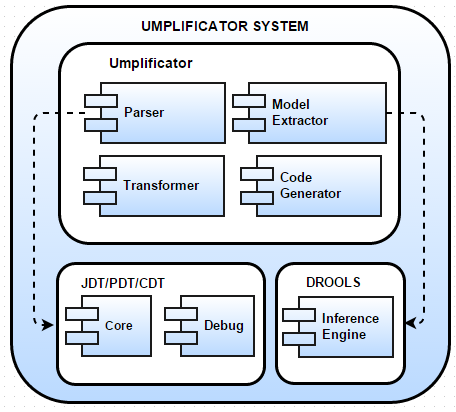
\includegraphics[width=0.75\textwidth]{Figures/UmplificatorComponents.png} 
\caption{The Umplificator components}
\label{fig:architecture}
\end{figure}

The mapping rules and rule engine are introduced in the following sub-section. 

\begin{figure}[h]
\centering
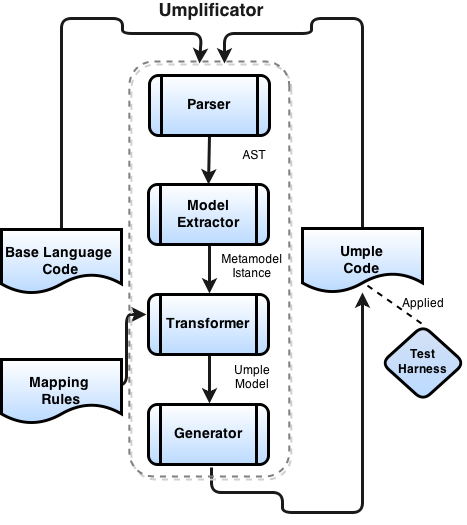
\includegraphics[width=0.75\textwidth]{Figures/Umplificator_ProcessFlow.png} 
\caption{The umplification process flow}
\label{fig:process_flow}
\end{figure}

\subsection{Rule Based Language}
The rule engine interprets and executes the mapping rules on the source model and target model to produce the umplified version of the target model.
The Drools engine used by the Umplificator is composed of an inference engine that is able to scale to a large number of rules and facts.  The inference component matches facts and data (base language models) against rules to infer conclusions, which result in actions (model transformations). A rule is a two-part structure (LHS and RHS) using first order logic for reasoning over knowledge representation. Pattern matching is performed to match facts against rules and is implemented using the Rete algorithm [15]. The rule engine is initialized with the rules. A Drools rule has the basic form: 

\begin{lstlisting}[language={drools},label={lst:drools}, caption=Basic rule in Drools] 
rule "name" 
  when LHS then RHS
end
\end{lstlisting}


where LHS is the conditional part of the rule and RHS is a block that allows dialect-specific semantic code to be executed. 
The rules are grouped in files for each of the cases (levels of refactoring) discussed earlier. In other words, there is a rule file containing rules, functions and queries to transform variables into attributes, another file containing those to transform variables into associations and so on. 
The rules as explained in this paper are instructions indicating how a piece of the Base language model (Java Model, C++ model, etc.) is mapped to a piece of an Umple model. Additionally, in Drools, one can specify:
\begin{itemize}
\item \textbf{Functions}: These are used for invoking actions on the consequence (then) part of the rule, especially if that particular action is used over and over again. In the Umplificator, functions are used instead of helper classes so the logic is kept in one place.
\item \textbf{Queries}: These provide a means to search working memory and store the results under a named value. In the Umplificator, they are used to gather metric information about the models analyzed. For instance, a query numberOfPublicMethods(..) returns the number of methods having 'public' as modifier. Queries do not have side effects, meaning that their evaluation cannot alter the state of the corresponding executing unit. 
\end{itemize}

In the Umplificator, the logic used for model transformations resides in the rules. Moreover, by using rules, we have a single point of truth, a centralized repository of knowledge. Rules can be also read and understood easily, so they can also serve as documentation.
Traditionally, rule engines have two methods of execution [16]: forward chaining and backward chaining. In forward chaining, the facts are asserted into working memory resulting in one or more rules being concurrently true and scheduled for execution. In backward chaining (goal driven), one starts with a conclusion, which the engine tries to satisfy. Drools is a Hybrid Chaining System because it implements both forward and back-ward mechanism. Our Umplificator uses the forward chaining method of operation in which the inference engine starts with facts, propagates through the rules, and produces a conclusion (e.g. a refactoring).  


As an example, consider the rules in Listing . The rule named transformImport(Lines 1-10) matches and converts any Import Declaration (Java Language) into an Umple depend construct. The dependency (Line 8) is then added to a matched Umple Class. The Umple Class is then put into the working memory (Line 9) so subsequent transformations can be made on the object (forward chaining). The rule named JavaFieldIsUmpleAttribute converts Java fields into basic Umple attributes. The attribute is then added to a matched Umple Class (Line 24). The attribute is put into the working memory (Line 25) so subsequent transformations can be made such as determining if the attribute is lazy or not. The rule named isLazyAttribute, not shown here, is used for this purpose. This rule matches and converts any basic attribute (in memory) that conforms to the required conditions into a lazy attribute (e.g. attribute.setIsLazy(true)). The complete set of mapping rules for the umplificator can be found at the umple code repository [17].

\begin{lstlisting}[language={drools},label={lst:rule_import}, caption=Initial Refactoring Mapping Rules]
 rule  "transform_Import"
 when
  import: ImportDeclaration();
  uClass: UmpleClass() ;
 then
  Depend depend = new Depend(getImportName(import));
  uClass.addDepend(depend);
  insert(uClass);
end
\end{lstlisting}



 % The Umplificator Technologies

\chapter{Evaluation}
 % Evaluation

\lhead{\emph{\leftmark}}  
\chapter{Related Work}
 % Related Work

\chapter{Conclusions and Contributions}
\lhead{\emph{\leftmark}}  % Set the left side page header to 
In this thesis we presented our reverse engineering approach called Umplification and the corresponding prototype tool, the Umplificator. Umplification is the process of transforming step-by-step a base language program to an Umple program. The major advantages, compared to other approaches, are the concept of incrementality and the mapping rules, which we in-tend to make general-purpose and easy to modify and add.  
We presented some evaluation results showing that our approach and its current implementation are effective and efficient enough to be applied in the future to real systems. 
Key contributions of this work are expected to be the following:
\begin{enumerate}
\item The overall concept of umplification
\item An understanding of how umplification compares with other reverse engineering techniques (incrementality, minimal adjustment of code to prevent disruption)
\item The Umplificator tool itself
\item Case studies of Umplification, demonstrating strengths, weaknesses and opportunities, as well as hopefully demonstrating that the resulting system is easier to under-stand and has less code.
\item Transformation patterns for (mapping rules) Umplification and the language for ex-pressing these. These should be general-purpose and easily modifiable to allow future researchers, and even end users, to add to them.
\item Detection of associations (of all different types) and state machines in a body of code. There is little successful work in this area in the literature.
\end{enumerate}

	As a future work, we plan to apply the approach to other open source systems, improve the mapping rules, improve the technology to allow Umple code to be input and add support for dynamic analysis for cases in which static analysis and parsing of the code is not enough to capture all the possible umplifiable concepts that can be derived from a program. We also want to integrate mapping rules for state machines and some popular soft-ware design patterns.

 % Conclusions and Contributions

%% ----------------------------------------------------------------
% Now begin the Appendices, including them as separate files

\addtocontents{toc}{\vspace{2em}} % Add a gap in the Contents, for aesthetics

\appendix % Cue to tell LaTeX that the following 'chapters' are Appendices

\chapter{Appendix}

	% Appendix Title

%\input{Appendices/AppendixB} % Appendix Title

%\input{Appendices/AppendixC} % Appendix Title

\addtocontents{toc}{\vspace{2em}}  % Add a gap in the Contents, for aesthetics
\backmatter

%% ----------------------------------------------------------------
\label{Bibliography}
\lhead{\emph{Bibliography}}  % Change the left side page header to "Bibliography"
\bibliographystyle{unsrtnat}  % Use the "unsrtnat" BibTeX style for formatting the Bibliography
\bibliography{Bibliography}  % The references (bibliography) information are stored in the file named "Bibliography.bib"

\end{document}  % The End
%% ----------------------------------------------------------------